
\chapter*{Poisson\rq s Equation: Iteration Methods}
\addcontentsline{toc}{chapter}{Poisson\rq  s Equation: Iteration Methods} 
In three dimensions, Poisson\rq s equation is given by
\begin{equation}\label{eq:91}
\frac{\partial^{2} V}{\partial x^{2}}+\frac{\partial^{2} V}{\partial y^{2}}+\frac{\partial^{2} V}{\partial z^{2}}=-\frac{\rho}{\epsilon_{0}}
\end{equation}
Poisson\rq s equation is used to describe the electric potential in a region of space
with charge density described by $ρ:^1$ You can solve the full 3D equation using
the technique we teach you in this lab, but we won’t make you do that here.
Instead, we’ll focus on geometries that are infinitely long in the $z$-dimension with
a constant cross-section in the $x - y$ plane. In these cases the z derivative goes to
zero, and Poisson\rq s equation reduces to
\begin{equation}\label{eq:92}
\frac{\partial^{2} V}{\partial x^{2}}+\frac{\partial^{2} V}{\partial y^{2}}=-\frac{\rho}{\epsilon_{0}}
\end{equation}
Note that by studying this equation we are also studying Laplace\rq s equation (Poisson\rq s equation with $\rho = 0$) and the steady state solutions to the diffusion equation
in two dimensions ($\partial T / \partial t = 0$ in steady state).


\section*{Finite difference form}
\addcontentsline{toc}{section}{Finite difference form}
The first step in numerically solving Poisson\rq s equation is to define a 2-D spatial grid. For simplicity, we\rq ll use a rectangular grid where the x coordinate is represented by $N_x$ values $x_j$ equally spaced with step size $h_x$ , and the y coordinate is represented by $N_y$ values $y_k$ equally spaced with step size hy . This
creates a rectangular grid with $N_x × N_y$ grid points, just as we used in Lab 6 for
the 2-d wave equation. We\rq ll denote the potential on this grid using the notation $V(x_j,y_k) = V_{j,k}$ \\
The second step is to write down the finite-difference approximation to the
second derivatives in Poisson\rq s equation to obtain a grid-based version of Poisson\rq s
equation. In our notation, Poisson\rq s equation is the represented by
\begin{equation}\label{eq:93}
\frac{V_{j+1, k}-2 V_{j, k}+V_{j-1, k}}{h_{x}^{2}}+\frac{V_{j, k+1}-2 V_{j, k}+V_{j, k-1}}{h_{y}^{2}}=-\frac{\rho_{j, k}}{\epsilon_{0}}
\end{equation}

This set of equations can only be used at interior grid points because on the edges
it reaches beyond the grid, but this is OK because the boundary conditions tell us
what $V$ is on the edges of the region.
\\
Equation \ref{eq:93} plus the boundary conditions represent a set of linear equations for the unknowns $V_{j,k}$ , so we could imagine just doing a big linear solve to
find $V$ all at once. Because this sounds so simple, let\rq s explore it a little to see why
we are not going to pursue this idea. The number of unknowns $V_{j,k}$ is $N_x × N_y$ ,
which for a 100 $×$ 100 grid is 10,000 unknowns. So to do the solve directly we would
have to be working with a 10,000 $×$ 10,000 matrix, requiring 800 megabytes of RAM
to store the matrix. Doing this big solve is possible for 2-dimensional problems
like this because computers with much more memory than this are common.
However, for larger grids the matrices can quickly get out of hand. Furthermore,
if you wanted to do a 3-dimensional solve for a 100 $×$ 100 $×$ 100 grid, this would
require $(10^4)^3 × 8 = 8 × 10^{12}$, or about 8 terabytes of memory. Computers like this
are becoming possible, but this is still a tiny computational grid. So even though
computers with large amounts of RAM are becoming common, people still use
iteration methods like the ones we are about to describe.

\section*{Iteration method on a simple example}
\addcontentsline{toc}{section}{Iteration method on a simple example}
Consider solving this equation:

\begin{equation}\label{eq:94}
x = e^{-x}
\end{equation}
One method to solve this equation is to make a guess for the solution, call it $x_0$,
and then iterate on the equation like this:
\begin{equation}\label{eq:95}
x_{n+1}=e^{-x_{n}}
\end{equation}
For large values of $n$, we find that the process converges to the exact solution
$ \bar{x} = 0.567$. Let\rq s do a little analysis to see why it works. Let $\bar{x}$ be the exact solution
of this equation and suppose that at the $n^{th}$ iteration level we are close to the
solution, only missing it by the small quantity $\delta n$ like this: $x_n = \bar{x} + \delta n$. Let\rq s
substitute this approximate solution into Eq. \ref{eq:95} and expand using a Taylor
series. Recall that the general form for a Taylor\rq s series is
\begin{equation}\label{eq:96}
f(x+h)=f(x)+f^{\prime}(x) h+\frac{1}{2} f^{\prime \prime}(x) h^{2}+\cdots+f^{(n)}(x) \frac{h^{n}}{n !}+\cdots
\end{equation}

When we substitute our approximate solution into 
Eq. \ref{eq:95} and 
expand around the exact solution $ \bar{x} $ we get

\begin{equation}\label{eq:97}
f(x_{n+1}=e^{-\bar{x}-\delta_{n}} \approx e^{-\bar{x}}-\delta_{n} e^{-\bar{x}}+\cdots
\end{equation}

If we ignore the terms that are higher order in $\delta$ (represented by ···), then Eq. \ref{eq:97}
shows that the error at the next iteration step is $\delta_{n+1} = −e^{−\bar{x}}\delta_n$. When we are close
to the solution the error becomes smaller every iteration by the factor $−e^{-\bar{x}}$. Since $\bar{x}$ is positive, $e^{-\bar{x}}$ is less than 1, and the algorithm converges. When iteration works
it is not a miracle—it is just a consequence of having this expansion technique
result in an error multiplier that is less than 1 in magnitude.

\begin{problem}\label{P9.1}
Write a program to solve the equation $x = e^{−x}$ by iteration and verify that
it converges. Then try solving this same equation the other way round:
$x = −ln x$ and show that the algorithm doesn\rq t converge. If you were to
use the $\bar{x} +\delta$ analysis above for the logarithm equation, you\rq d find that the
multiplier is bigger than one. Our time is short today, so we won\rq t make you
do this analysis now, but it is a good exercise if you want to look at it on
your own time.
\end{problem}

\section*{Iteration method on Poisson\rq s equation}
\addcontentsline{toc}{section}{Iteration method on Poisson\rq s equation}
	\marginpar{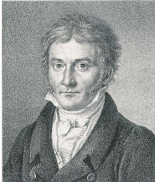
\includegraphics[width=\marginparwidth]{gauss} Friedrich Gauss (1777$-$1855, German) }
Well, what does this have to do with Poisson\rq s equation? If we solve the finitedifference version of Poisson\rq s equation (Eq. \ref{eq:93}) for $V_{j,k}$ , we find
\begin{equation}\label{eq:98}
f(x_{n+1}=e^{-\bar{x}-\delta_{n}} \approx e^{-\bar{x}}-\delta_{n} e^{-\bar{x}}+\cdots
\end{equation}
With the equation in this form we could just iterate over and over by doing the
following.

\begin{itemize}
\item Choose an initial guess for the interior values of $V_{j,k}$ .
\item Use this initial guess to evaluate the right-hand side of Eq. \ref{eq:98}
\item Replace our initial guess for $V_{j,k}$ by this right-hand side, and then repeat.

\end{itemize}
If all goes well, then after many iterations the left and right sides of this equation will agree and we will have a solution. \\
To see, let\rq s notice that the iteration process indicated by Eq. \ref{eq:98} can be
written in matrix form as
\begin{equation}\label{eq:99}
V_{n+1}=\mathbf{L} V_{n}+r
\end{equation}
where $L$ is the matrix which, when multiplied into the vector $V_n$, produces the
$V_{j,k}$ part of the right-hand side of Eq. \ref{eq:98} and $r$ is the part that depends on the
charge density $ \rho_{j,k}$ . (Don\rq t worry about what $L$ actually looks like; we are just
going to apply general matrix theory ideas to it.) As in the exponential-equation
example given above, let $\bar{V}$ be the exact solution vector and let $\delta_n$ be the error
vector at the $n^{th}$ iteration. The iteration process on the error is, then,
\begin{equation}\label{eq:910}
\delta_{n+1}=\mathbf{L} \delta_{n}
\end{equation}
Now think about the eigenvectors and eigenvalues of the matrix $L$. If the matrix is
well-behaved enough that its eigenvectors span the full solution vector space of
size $N_x × N_y$ , then we can represent $\delta n$ as a linear combination of these eigenvectors. This then invites us to think about what iteration does to each eigenvector. The answer, of course, is that it just multiplies each eigenvector by its eigenvalue.
Hence, for iteration to work we need all of the eigenvalues of the matrix $L$ to have
magnitudes less than 1.\\
So we can now restate the conditions for this approach to work: Iteration on
Eq. \ref{eq:98} converges if all of the eigenvalues of the matrix $L$ on the right-hand side
of Eq. \ref{eq:98} are less than 1 in magnitude. This statement is a theorem which can be
proved if you are really good at linear algebra, and the entire iteration procedure
described by Eq. \ref{eq:99} is known as Jacobi iteration. Unfortunately, even though
all of the eigenvalues have magnitudes less than 1 there are lots of them that have
magnitudes very close to 1, so the iteration takes forever to converge (the error
only goes down by a tiny amount each iteration). \\ 
But Gauss and Seidel discovered that the process can be accelerated by making
a very simple change in the process. Instead of only using old values of $V_{j,k}$ on
the right-hand side of Eq. \ref{eq:98}, they used values of $V_{j,k}$ as they became available
during the iteration. (This means that the right side of \ref{eq:98} contains a mixture
of $V$ -values at the $n$ and $n +1$ iteration levels.) This change, which is called GaussSeidel iteration is really simple to code; you just have a single array in which to
store $V_{j,k}$ and you use new values as they become available. Here as a coded
example of Guass-Seidel iteration for a rectangular region grounded on two sides,
with the two other sides held at a potential:
\begin{lstlisting}
from mpl_toolkits.mplot3d import Axes3D
import matplotlib.pyplot as plt
import numpy as np

# Make the grid
xmin = 0
xmax = 2
Nx = 80
x,hx = np.linspace(xmin,xmax,Nx,retstep = True)
hx2 = hx**2

ymin = 0
ymax = 2
Ny = 40
y,hy = np.linspace(ymin,ymax,Ny,retstep = True)
hy2 = hy**2
X,Y = np.meshgrid(x,y,indexing='ij')

# Initialize potential
V = 0.5*np.ones_like(X)

# Enforce boundary conditions
V[:,0] = 0

V[:,-1] = 0
V[0,:] = 1
V[-1,:] = 1

# Allow possibility of charge distribution
rho = np.zeros_like(X)

# Iterate
denom = 2/hx2 + 2/hy2
fig = plt.figure(1)
for n in range(200):
	# make plots every few steps
	if n % 10 == 0:
		plt.clf()
		ax = fig.gca(projection='3d')
		surf = ax.plot_surface(X,Y,V)
		ax.set_zlim(-0.1, 2)
		plt.xlabel('x')
		plt.ylabel('y')
		plt.draw()
		plt.pause(0.1)

	# Iterate the solution
	for j in range(1,Nx-1):
		for k in range(1,Ny-1):
			V[j,k] = ( (V[j+1,k] + V[j-1,k])/hx2
				+(V[j,k+1] + V[j,k-1])/hy2
				+rho[j,k]) / denom
\end{lstlisting}
\begin{problem}\label{P9.2}  Paste the code above into a program, run it, and watch the solution iterate.
Study the code, especially the part in the loop. When you understand the
code, call a TA over and explain it to them to pass off this part.
\end{problem}

\section*{Successive over-relaxation}
\addcontentsline{toc}{section}{Successive over-relaxation}
Gauss-Seidel iteration is not the best we can do, however. To understand the next
improvement let\rq s go back to the exponential example

\begin{equation}\label{eq:911}
x_{n+1}=e^{-x_{n}}
\end{equation}
and change the iteration procedure in the following non-intuitive way:
\begin{equation}\label{eq:912}
x_{n+1}=\omega e^{-x_{n}}+(1-\omega) x_{n}
\end{equation}
where $\omega$ is a number which is yet to be determined.
\begin{problem}\label{P9.3}Verify quickly on paper that even though Eq. \ref{eq:912} looks quite different
from Eq. \ref{eq:911}, it is still solved by $x = e^{-x}$.\end{problem}
If we insert xn = x¯ + δn into this new equation and expand as before, the error
changes as we iterate according to the following
\begin{equation}\label{eq:913}
x_{n+1}=\omega e^{-x_{n}}+(1-\omega) x_{n}
\end{equation}

Notice what would happen if we chose $\omega$ so that the factor in parentheses were
zero: The equation says that we would find the correct answer in just one step! Of
course, to choose $\omega$ this way we would have to know $\bar{x}$, but it is enough to know
that this possibility exists at all. All we have to do then is numerically experiment
with the value of $\omega$ and see if we can improve the convergence.

\begin{problem}\label{P9.4} Write a program that accepts a value of $\omega$ and runs the iteration in Eq. \ref{eq:912}.
Experiment with various values of $\omega$ until you find one that does the best
job of accelerating the convergence of the iteration. You should find that
the best $\omega$ is near 0.64, but it won’t give convergence in one step. See if you
can figure out why not.\\
Hint: Think about the approximations involved in obtaining Eq. \ref{eq:913}. Specifically go back to the previous derivation and look for terms represented by dots.\\
\end{problem}
As you can see from Eq. \ref{eq:913}, this modified iteration procedure shifts the
error multiplier to a value that converges better. So now we can see how to
improve Gauss-Seidel: we just use an $\omega$ multiplier like this:
\begin{equation}\label{eq:914}
V_{n+1}=\omega\left(\mathbf{L} V_{n}+r\right)+(1-\omega) V_{n}
\end{equation}
then play with $\omega$ until we achieve almost instantaneous convergence. \\ 
Sadly, this doesn\rq t quite work. The problem is that in solving for $N_x × N_y$
unknown values $V_{j,k}$ we don\rq t have just one multiplier; we have one for each
eigenvalue of the matrix. So if we shift one of the eigenvalues to zero, we might
shift another one to a value with magnitude larger than 1 and the iteration will
not converge at all. The best we can do is choose a value of $\omega$ that centers the
entire range of eigenvalues symmetrically between −1 and 1. \\ 
Using an $\omega$ multiplier to shift the eigenvalues is called Successive OverRelaxation, or SOR for short. Here it is written out so you can code it:
\begin{equation}\label{eq:915}
V_{j, k}=\omega\left(\frac{V_{j+1, k}+V_{j-1, k}}{h_{x}^{2}}+\frac{V_{j, k+1}+V_{j, k-1}}{h_{y}^{2}}+\frac{\rho_{j, k}}{\epsilon_{0}}\right) /\left(\frac{2}{h_{x}^{2}}+\frac{2}{h_{y}^{2}}\right)+(1-\omega) V_{j, k}
\end{equation}
And what value should we use for $\omega$? The answer is that it depends on the values
of $N_x and N_y$ . In all cases ω should be between 1 and 2, with $\omega = 1.7$ being a
typical value. Some wizards of linear algebra have shown that the best value of $\omega$ when the computing region is rectangular and the boundary values of $V$ are fixed (Dirichlet boundary conditions) is given by
\begin{equation}\label{eq:916}
\omega=\frac{2}{1+\sqrt{1-R^{2}}}
\end{equation}
where
\begin{equation}\label{eq:917}
R=\frac{h_{y}^{2} \cos \left(\pi / N_{x}\right)+h_{x}^{2} \cos \left(\pi / N_{y}\right)}{h_{x}^{2}+h_{y}^{2}}
\end{equation}
These formulas usually give a reasonable estimate of the best $\omega$ to use. Note,
however, that this value of $\omega$ was found for the case of a cell-edge grid with the
potential specified at the edges. If you use a cell-centered grid with ghost points,
and especially if you change to derivative boundary conditions, this value of $\omega$
won\rq t be quite right. But there is still a best value of $\omega$ somewhere near the value
given in Eq. \ref{eq:916} and you can find it by numerical experimentation. \\ 
Finally, we come to the question of when to stop iterating. It is tempting just to watch the values of $V_{j, k}$ and quit when the values stabilize at some level, like this for instance: quit when $\epsilon=\left|V(j, k)_{n+1}-V(j, k)_{n}\right|<10^{-6}$. You will see this error criterion sometimes used in books, but do not use it. We know of one person who published an incorrect result in a journal because this error criterion lied. We done\rq t want to quit when the algorithm has quit changing $V$; we want to quit when Poisson\rq s equation is satisfied. (Most of the time these are the same, but only looking at how $V$ changes is a dangerous habit to acquire.) In addition, we want to use a relative (\%) error criterion. This is easily done by setting a scale voltage $V_{\text {scale }}$ which is on the order of the biggest voltage in the problem and then using for the error criterion
\marginpar{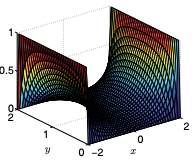
\includegraphics[width=\marginparwidth]{fig91}\captionof{figure}{The electrostatic potential $V(x, y)$ with two sides grounded and two sides at constant potential.}\label{fig:43}}

\begin{equation}\label{eq:918}
\epsilon=\left|\frac{\text { Lhs }-\mathrm{Rhs}}{V_{\text {scale }}}\right|
\end{equation}
where Lhs is the left-hand side of Eq. \ref{eq:98} and Rhs is its right-hand side. Because this equation is just an algebraic rearrangement of our finite-difference approximation to Poisson\rq s equation, $\epsilon$ can only be small when Poisson\rq s equation is satisfied. (Note the use of absolute value; can you explain why it is important to use it? Also note that this error is to be computed at all of the interior grid points. Be sure to find the maximum error on the grid so that you only quit when the solution has converged throughout the grid.)\\

And what value should we choose for the error criterion so that we know when to quit? Well, our finite-difference approximation to the derivatives in Poisson\rq s equation is already in error by a relative amount of about $1 /\left(12 N^{2}\right)$, where $N$ is the smaller of $N_{x}$ and $N_{y}$. There is no point in driving $\epsilon$ below this estimate. For more details, and for other ways of improving the algorithm, see Numerical Recipes, Chapter $19 .$

\begin{problem}\label{P9.5}
Starting with the Gauss-Seidel example above, implement all of the improvements described above to write a full successive over-relaxation routine. Note that you will need to replace the $for$ loop on the variable $n$ into a while loop that is based on the error criterion. Also move the plot command out of the loop so it only executes once, after the solution has converged. (So that you don\rq t have to wait for a bunch of plots to be drawn.) Run your code for a spatial region of size $L_{x}=4$ in the x-dimension and $L_{y}=2$ the $\mathrm{y}$-dimension arranged as shown in Fig. 9.1. Use $\mathrm{Nx}=\mathrm{Ny}=30$ and several different values of $\omega$. Note that the boundary conditions on the potential $V(x, y)$ are $V\left(-L_{x} / 2, y\right)=V\left(L_{x} / 2, y\right)=1$ and $V(x, 0)=V\left(x, L_{y}\right)=0$. Set the error criterion to $10^{-4}$. Verify that the optimum value of $\omega$ given by Eq. \ref{eq:916} is the best one to use.
\end{problem}

\section*{Some Different Geometries}
\addcontentsline{toc}{section}{Some Different Geometries}

\begin{problem}\label{P9.6}
	\marginpar{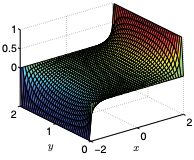
\includegraphics[width=\marginparwidth]{fig92}\captionof{figure}{The potential $V(x, y)$ rom Problem \ref{P9.6}(a).}\label{fig:44}}
		\marginpar{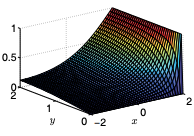
\includegraphics[width=\marginparwidth]{fig93}\captionof{figure}{The potential $V(x, y)$ with zero-derivative boundary conditions on two sides (Problem \ref{P9.6}(b).)}\label{fig:45}}
\begin{enumerate}[label=(\alph*)]
\item Modify your code to model a rectangular pipe with $V(x=-2, y)=-1$, $V(x=2, y)=1$, and the $y=0$ and $y=L_{y}$ edges held at $V=0$.
\item Modify your code from (a) so that the boundary condition at the $x=$ $-L_{x} / 2$ edge of the computation region is $\partial V / \partial x=0$ and the boundary condition on the $y=L_{y}$ edge is $\partial V / \partial y=0$. You can do this problem either by changing your grid and using ghost points or by using a quadratic extrapolation technique (see Eq. \ref{eq:210}). Both methods work fine, but note that you will need to enforce boundary conditions inside the main SOR loop now instead of just setting the values at the edges and then leaving them alone.
You may discover that the script runs slower on this problem. See if you can make it run a little faster by experimenting with the value of $\omega$ that you use. Again, changing the boundary conditions can change the eigenvalues of the operator. (Remember that Eq. (9.16) only works for cell-edge grids with fixed-value boundary conditions, so it only gives a ballpark suggestion for this problem.)
\item Study electrostatic shielding by going back to the boundary conditions of Problem \ref{P9.6}(a), while grounding some points in the interior of the full computation region to build an approximation to a grounded cage. Allow some holes in your cage so you can see how fields leak in. First make a rectangular cage similar to Fig. 9.4, but then you can try other geometries.
You will need to be creative about how you build your cage and about how you make SOR leave your cage points grounded as it iterates. One thing that won\rq t work is to let SOR change all the potentials, then set the cage points back to $V=0$ before doing the next iteration. This takes forever to converge. It is much better to set them to zero and force SOR to never change them. An easy way to do this is to use a cell-edge grid with a mask. A mask is an array that you build that is the same size as $V$, initially defined to be full of ones like this
\begin{lstlisting}
mask = np.ones_like(V)
\end{lstlisting}
Then you go through and set the elements of mask that you don't want SOR to change to have a value of zero. (We'll let you figure out the logic to do this for the cage.) Once you have your mask built, you add an if statement to our code so that the SOR stuff inside the $j$ and $k$ for loops only changes a given point and updates the error if $\operatorname{mask}(j, k)$ is one. This logic assumes you have to set the values of $V$ for these points before the for loop execute, just like the boundary conditions. Using this technique you can calculate the potential for quite complicated shapes just by changing the mask array.
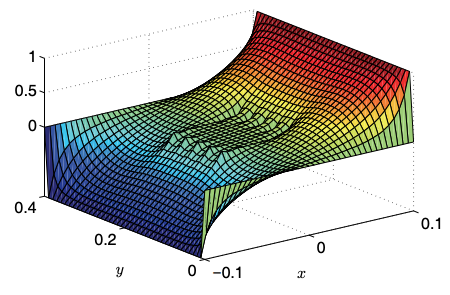
\includegraphics[width=0.7\textwidth]{fig94}\captionof{figure}{The potential $V (x, y)$ for an electrostatic \rq\rq cage\lq\lq formed by
grounding some interior points. (Problem \ref{P9.6}(c).)}
\end{enumerate}
\end{problem}
